\documentclass[a4paper]{article}

%% Language and font encodings
\usepackage[english]{babel}
\usepackage[utf8]{inputenc}
\usepackage[T1]{fontenc}

%% Sets page size and margins
\usepackage[a4paper,top=3cm,bottom=2cm,left=3cm,right=3cm,marginparwidth=1.75cm]{geometry}

%% Useful packages
\usepackage{amsmath}
\usepackage{graphicx}
\usepackage[colorinlistoftodos]{todonotes}
\usepackage[colorlinks=true, allcolors=blue]{hyperref}
\usepackage{csvsimple}

\newcommand{\github}{https://github.com/kauron/etsinf3/tree/master/CPA/lab2}

\title{CPA Lab 2}
\author{Carlos Santiago Galindo Jiménez\\Jesús Vélez Palacios}

\begin{document}
\maketitle
\section{Objective}
Parallelize the execution of a program that reconstructs an image whose rows have been shuffled. Study different approaches and some improvements to the algorithm.

\section{Exercices}
\begin{description}
    \item [\texttt{\href{\github /src/encaja-e1.c\#L167}{encaja-e1.c}}] Time the method encaja. Completed with two calls to \texttt{omp\_get\_wtime()}.
    \item [\texttt{encaja-e2-p?.c}] Parallelize the different loops (if at all possible).
    \begin{description}
        \item [\texttt{i}] This loop will never be parallelizable, because each line depends on the previous one.
        \item [\texttt{j}] This loop can be parallalelized protecting the variables with \texttt{private(x, distancia)}. The last \texttt{if} must be protected as \texttt{critical section} and the condition has to be rechecked after entering it. \href{\github /src/encaja-e2-pJ.c\#L118}{Source code}
        \item [\texttt{x}] This loop can also be parallelized, and needs a \texttt{reduction(+:distancia)} to compute the distance correctly. \href{\github /src/encaja-e2-pX.c\#L120}{Source code}
    \end{description}
    \item [\texttt{\href{\github /src/encaja-e3.c\#L122}{encaja-e3.c}}] Improve the program by exiting loop \texttt{x} if the partial sum surpasses the current minimum. Solved adding an \texttt{if} that breaks from the loop in that case.
    \item [\texttt{encaja-e4-p?.c}] Parallelize \texttt{encaja-e3.c} in the loops that are viable.
    \begin{description}
        \item [\texttt{j}] This loop is parallelized in the same way as in exercise 2. \href{\github /src/encaja-e4-pJ.c\#L118}{Source code}
        \item [\texttt{x}] This loop needs the most work. It must be parallelized as a \texttt{parallel} block. The first iteration is assigned to \texttt{omp\_get\_thread\_num()} and each thread increments \texttt{x} by \texttt{omp\_get\_num\_threads()}. It still needs a \texttt{reduction} for \texttt{distancia}. \href{\github /src/encaja-e4-pX.c}{Source code}
    \end{description}
\end{description}

\section{Performance}

\subsection{Timing}
The sequential programs (\texttt{encaja-e1.c} and \texttt{encaja-e3.c}) have only been tested once. The parallel programs have been run with 2, 4, 8, 16 and 32 threads available to test their performance. As shown in the graph from Figure 3, loop \texttt{j} achieves much better results that loop \texttt{x}. On top of that, the improvement implemented in the exercises 3 and 4 pays off in the sequential version, but less and less as the number of threads grows bigger.

\begin{figure}[h]
    \centering
    \begin{tabular}{l r}
        Program            & Execution time \\ \hline
        \texttt{encaja-e1} & 15.257217      \\
        \texttt{encaja-e3} &  2.725587      \\
    \end{tabular}
    \caption{Sequential execution times}
\end{figure}
\begin{figure}[h]
    \centering
    \begin{tabular}{l r r r r r}
        Program               & 2t        & 4t        & 8t        & 16t        & 32t        \\ \hline
        \texttt{encaja-e2-pJ} & 6.938746  & 3.548883  & 1.970450  & 1.183996   & 0.726187   \\
        \texttt{encaja-e2-pX} & 8.337415  & 5.464151  & 5.557857  & 8.197272   & 12.789012  \\
        \texttt{encaja-e4-pJ} & 1.439842  & 0.795035  & 0.496000  & 0.330912   & 0.256960   \\
        \texttt{encaja-e4-pX} & 4.065065  & 4.217589  & 5.164125  & 8.656438   & 13.590685  \\
    \end{tabular}
    \caption{Parallel execution times}
\end{figure}

\begin{figure}[h]
    \centering
    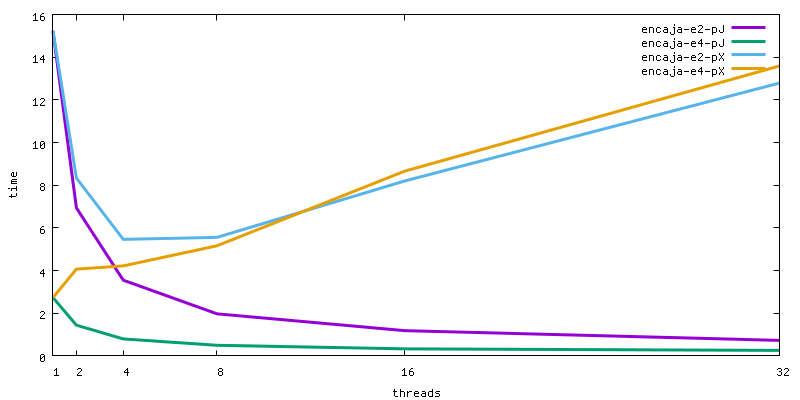
\includegraphics[width=\textwidth]{../img/time}
    \caption{Threads\, \textemdash \unskip \, time graph \protect\footnotemark }
\end{figure}

\footnote{The data in the graph for $nodes=1$ is the timing from the sequential versions of the program (\texttt{encaja-e1.c} and \texttt{encaja-e3.c})}

\subsection{Speedup}
The speedup of a parallel program respect to the sequential version is the improvement (or not) of the parallel version out of one, and it is computed as:
$$S(n,p)=\frac{t(n)}{t(n,p)}$$
Applying the previous formula to the tables we obtain these. \todo[inline]{Analyse data!}

\todo[inline]{insert tables}
\begin{figure}[h]
    \centering
    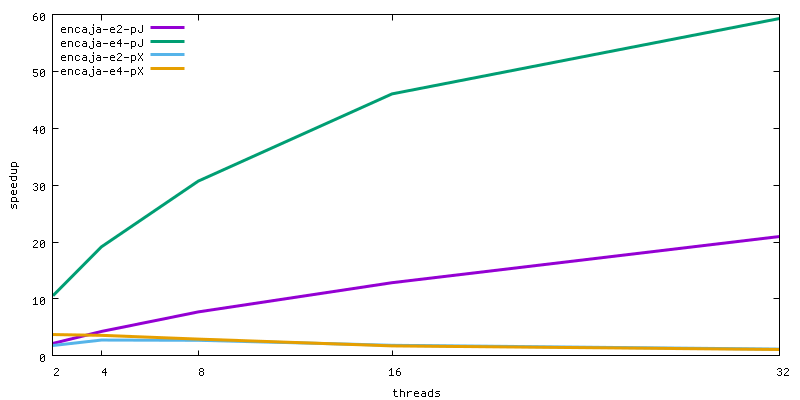
\includegraphics[width=\textwidth]{../img/speedup}
    \caption{Threads\, \textemdash \unskip \, speedup graph}
\end{figure}

\subsection{Efficiency}
\todo[inline]{introduce}
$$E(n,p)=\frac{S(n,p)}{p}$$
\todo[inline]{introduce tables/graph and analyse data}

\todo[inline]{insert tables}
\begin{figure}[h]
    \centering
    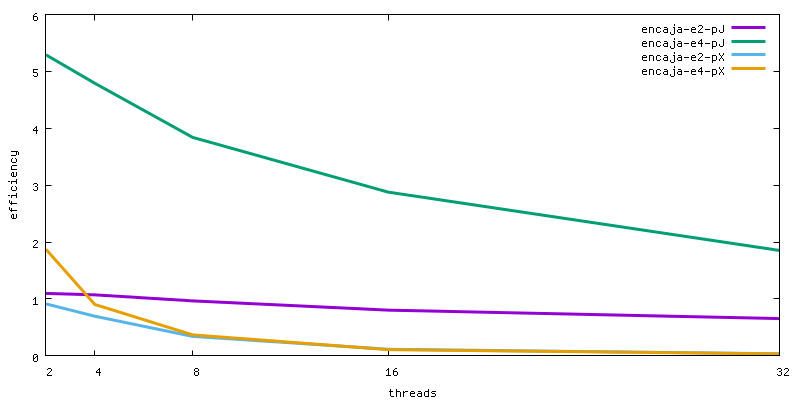
\includegraphics[width=\textwidth]{../img/efficiency}
    \caption{Threads\, \textemdash \unskip \, efficiency graph}
\end{figure}

\section{Conclussions}
\todo[inline]{write conclussions}


\end{document}

